% #############################################################################
% This is Chapter 1
% !TEX root = ../main.tex
% #############################################################################
% Change the Name of the Chapter i the following line
\fancychapter{Introduction}
\cleardoublepage
% The following line allows to ref this chapter
\label{chap:intro}

	The act of making something as fully perfect, functional or effective as possible is a behavior that is constantly sought by us, Humans, in a process known as optimization ~\cite{MerriamWebster2017OptimizationDefinition}. Intuitively, through optimization one aims to improve a system in terms of different quantitative measurable aspects. Although usually striving to fully optimize these systems, i.e., to obtain \textit{perfect} systems, it is often the case, that finding a better one or a near-optimal system suffices.

	Generally, optimization processes are composed of two main parts: (1) the model of the system to be optimized and (2) the algorithm responsible for finding the optima. Conceptually, the model is a description of the system that is defined in terms of: a set of the system's characteristics, known as variables or unknowns, a set of quantitative measures of the system's performance, referred to as objectives or criteria, and, optionally, by a set of conditions that have to be satisfied to guarantee the system's feasibility, i.e., the system's constraints~\cite{Nocedal2011NumericalOptimization}. The objectives are usually functions of the variables being defined. Subsequent to the model definition, the obtained description can be interpreted as an optimization problem for which the optimal solutions are to be found, thus entering in the second part of an optimization process. In the second part, one executes an optimization algorithm, which encloses a description of the steps necessary to attain optimal solutions, which according to the user's intentions can be the maximization or minimization of the model's objectives.

	Depending on the model representation, one is able to classify optimization problems differently with respect, for example, to its objective functions, variables, and determinacy. Due to their relevance in the developed work, in the next two paragraphs, we describe four different optimization classifications. However, we refer the interested reader to~\cite{Nocedal2011NumericalOptimization} for a more detailed and complete description of the different classifications.

	One important classification is regarding the cardinality of the solutions sought by optimization processes, thus yielding the continuous and discrete optimization categories. In the former, optimal solutions lie in a potentially infinite set of candidate solutions, whereas in the latter, optimal solutions lie in a finite set. Optimization problems can also be classified as constrained or unconstrained, depending on whether the models explicitly define constraints or not. Moreover, optimization can also be distinguished in terms of the aim of the search that is performed, particularly, whether it is global or local. In local optimization, the search process strives to find a solution that is locally optimal, i.e., for which its value is better than all other points in its vicinity. The points that satisfy the previous property are known as local optima. On the other hand, there are optimization processes that strive to find the globally optimal solutions, i.e., the best of all the local optima.

	Optimization is frequently required to address problems involving more than one objective. It is often the case that people face daily decisions involving two or more conflicting objectives, either to effectively manage resources, or just to ponder several factors associated with certain decisions. \todo{[Buyers dilemma, falar de computadores» CPU + RAPIDO, mas fica sem energia mais rapido...] When buying a new car, one often must simultaneously consider conflicting aspects, such as its speed, its style, and its economy: a faster car is usually less economic, a more aesthetically pleasant car is usually less economic, and a more economic car is hardly ever faster or fashionable.} This example belongs to the subset of \ac{MOO} problems which considers the optimization of more than one objective function. 

	In addition to day-to-day life decisions, optimization can also be used with different decision and analysis purposes. As a result, several areas, including economy, science, engineering, among others apply optimization as auxiliary tool to maximize the efficiency of the decisions involved. Particularly, architecture is one of the areas where the potential of optimization becomes more visible. The architectural practice can benefit from optimization to reduce the building sector's economic and ecological footprint through the finding of more efficient buildings variants before their construction. Given its importance to the world's sustainability and economy, this thesis focus on the application of optimization processes to enhance the architectural practice, providing, in the following sections, an overview of the involvement and the evolution of such processes in architecture. We end this chapter by highlighting our research goals and by outlining the upcoming document's structure.

%% #############################################################################
\section{From design to Optimized design}
	
	The usefulness of optimization goes beyond architectural design applications, benefiting other engineering fields like Mechanics or Electronics, through the optimization of its components and circuits designs, respectively. 
	
	In the architectural practice, optimization has been gaining relevance for the past few years~\cite{Cichocka2017SURVEY}, especially due to the impact of building construction and building maintenance in the economy and environment. For this reason, designers are shifting from a pure aesthetically-based to performance-based design, where buildings are being optimized to achieve the best possible values regarding different aspects of their design, such as thermal comfort, energy consumption, lighting comfort, structural behavior, cost, among others.

	This has only been possible due to the technological improvements in the architectural practice over the last few decades. The adoption of computer science techniques was responsible for the dissemination of digital modelling tools, which allowed the more accurate and efficient design of highly complex buildings. These tools enabled a shift from traditional paper-based approaches to more computerized ones, such as \ac{CAD} and \ac{BIM} applications, where changes to designs are trivial and do not require manually erasing and redrawing parts of the original design~\cite{Ferreira2015GD}.~\Cref{fig:traditionaldesign} illustrates the general view of this computer-aided design process, as well as an example of a 3D modeling tool. The architect interacts directly with these modeling tools to incrementally concretize his design ideas.
	
\begin{figure*}[htbp]
\centering
\subfigure[]{%
\label{fig:traditionaldesign-a}%

\includegraphics[width=0.38\textwidth]{./Images/Introduction/TraditionalArchitecturalDesign.png}}%
\hfill
\subfigure[]{%
\label{fig:traditionaldesign-b}%
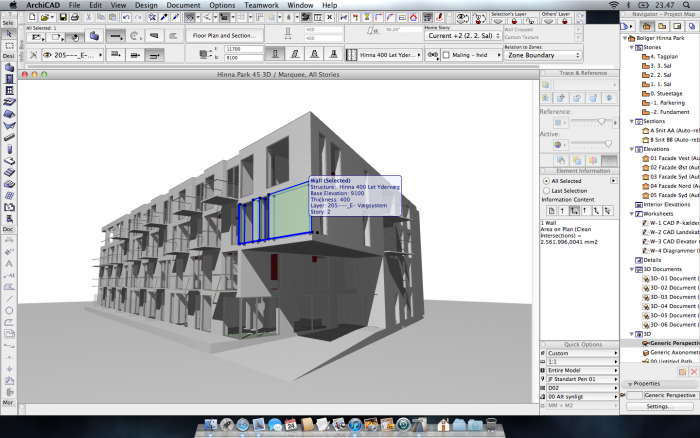
\includegraphics[width=0.48\textwidth]{./Images/Introduction/Example3DModellingTool_1.png}}%

\caption[General views of Traditional Design Approaches]{(a) Computer-aided design workflow (b) Building design example in a 3D modeling tool}
\label{fig:traditionaldesign}
\end{figure*}

	Shortly after, the development of computer-based simulation tools allowed designers to simulate their building's behavior regarding specific criteria, and, thus get a measurement of its performance~\cite{Malkawi2005}. Through this process, called \ac{BPS}, designers could easily validate whether their building's performance satisfied the efficiency requirements and, ultimately, optimize their design by iteratively generating multiple variations of the same design, assessing their performance, and selecting the better ones. Albeit being very primitive, architects now had the elementary mechanisms required for optimizing their building's designs.

% #############################################################################
\subsection{Building Performance Optimization}

	\ac{BPO}, a simulation-based optimization approach, treats the results produced by the simulation tool as the functions to optimize. Although invariably suffering from some degree of imprecision and inaccuracy, using these simulations it becomes possible to estimate the performance of complex designs. Particularly, these estimates are beneficial in designs for which analytical solutions are often very difficult or even impossible to derive~\cite{Kolda2003}. In these cases, the objective function, i.e., the function to optimize, is derived from the simulations' results. These objective functions have a domain which corresponds to the range of acceptable designs as specified by the architect.

	A known drawback of simulation-based approaches is the time required to achieve reasonable results for complex systems~\cite{Law1991} which is associated with different aspects of the problem, namely (1) its \textbf{domain} which, depending on the nature of the problem, might use different methodologies to produce the corresponding estimates (e.g., thermal \textit{versus} structural); (2) its \textbf{intrinsic structure} which, depending on the attributes and relations of the system, might lead either to simpler or to more complicated computations (e.g., skyscraper \textit{versus} a small house); and (3) its \textbf{analytical model}, which has the essential properties of the system we are trying to simulate and that will be used as input to the simulation tool. Generally, the domain and structure do not change for the same problem, albeit there are numerous ways to produce multiple analytical models. Depending on the level of detail of the analytical model, both the computational time and the result of the simulation might change. \todo{Dar exemplo??}

	In architecture, the generation of each analytical model is a time-consuming and complicated task. On the one hand, it is often necessary to generate multiple models of the same design because of the simulation tools' specificity, i.e., in order to evaluate a design, each simulation tool requires a specialized model of the same design. On the other hand, simulation tools often yield time-consuming processes, where a single simulation can take up to seconds, minutes, hours, days, or even weeks to complete. 
	
	In addition to the simulations' specificity and complexity, architectural designs are inherently complex, thus leading to less predictable objective functions, for which mathematical forms are difficult to formulate~\cite{Machairas2014}. For this reason, information about the derivatives of such functions cannot be extracted and methods depending on function derivatives cannot be used to address architectural optimization problems. As a result, classical gradient-based optimization methods can not be used. Instead, other methods that do not rely on the existence of an explicit mathematical form should be used, i.e., methods that treat the optimization functions as black-boxes, relying uniquely on the outputs of numerical simulations.
	
% Motivation for other design alternatives
	Despite the flexibility provided by \ac{CAD} and \ac{BIM} tools, architects often face difficulties when modeling complex geometry. A \ac{BPO} methodology requires to experiment with different design variations, which implies spending a large amount of time to manually make changes to the design. Since an optimization process requires evaluating several variations of the same design, the manual execution of the required changes implies a lot of effort, hence making the whole optimization process unviable.
	
% #############################################################################
\subsection{Algorithmic Design}

% Introduction to AD, way of overcoming limitations of manual approaches
	An approach capable of creating forms through algorithms is crucial for overcoming the aforementioned limitations. An example of an algorithm approach is the \ac{AD} approach~\cite{Branco2017AD}, which is depicted in \Cref{fig:algorithmicdesign}. In this approach, the architect entails an algorithmic description of the intended design. After elaborating the algorithm, executing it will automatically generate the corresponding 3D model in a \ac{CAD} or \ac{BIM} tool. Algorithmic approaches are inherently parametric, thus enabling the generation of different variations of the same design by making simple modifications to the values of the parameters~\cite{Leitao2014GD}. 
	
\begin{figure}[htbp]
\centering

\includegraphics[width=0.70\textwidth]{./Images/Introduction/AlgorithmicArchitecturalDesign.png}
\caption[General view of the Algorithmic Design Approach]{Algorithmic-based design workflow}
\label{fig:algorithmicdesign}
\end{figure}
	
	As an example consider the  algorithmic design of the Astana's National Library from BIG architects, illustrated in~\Cref{fig:astana-a}. Initially, the architect selects an \ac{AD} tool providing the necessary design primitives. Then, he uses these primitives to create a computational program enclosing the relative relations among the different design elements, so that when a modification occurs in one element, that modification is propagated throughout that element's dependencies. In the end, the architect creates a procedure responsible for creating the whole design \texttt{astana(radius, nturns)}, which when executed will produce the corresponding Astana 3D model. Using this procedure, he can easily generate different variations of the Astana by simply setting different values for the parameters: \texttt{radius}, defining the width of the whole design, and \texttt{nturns}, defining the number of turns in the design. \Cref{fig:astana} illustrates the original design and two design variations are represented: (a) the original design (b) design variation generated by doubling the radius of the original design, and (c) design variations generated by doubling the number of turns.
	
\begin{figure*}[htbp]
\centering
\subfigure[]{%
\label{fig:astana-a}%
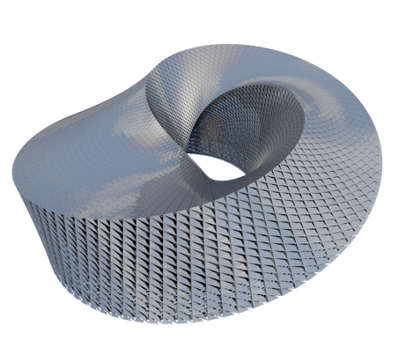
\includegraphics[width=0.32\textwidth]{./Images/Astana/Astana1.png}}%
\hfill
\subfigure[]{%
\label{fig:astana-b}%
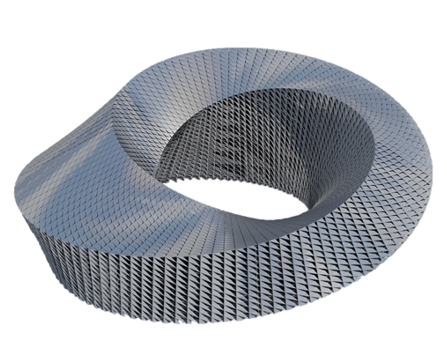
\includegraphics[width=0.33\textwidth]{./Images/Astana/Astana2.png}}%
\hfill
\subfigure[]{%
\label{fig:astana-c}%
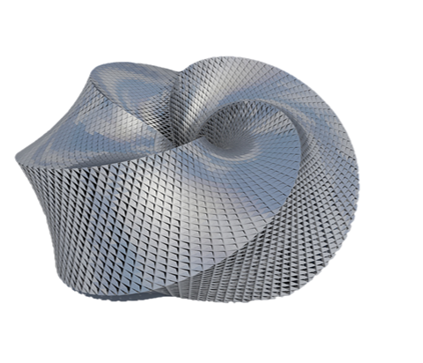
\includegraphics[width=0.33\textwidth]{./Images/Astana/Astana3.png}}%

\caption[Design variations of the Astana's National Library]{Astana's National Library Design variations: (a) Original (b) Larger diameter (c) Two Moebius Turns}
\label{fig:astana}
\end{figure*}

% Advantages over Manual approaches & Disadvantages
Only recently has the algorithmic paradigm begun to settle in the architectural practice. The requirement for programming knowledge is often an obstacle to the adoption of these approaches, since it requires larger initial investments for the architect to learn how to program. Despite the larger initial investments, the benefits obtained with algorithmic approaches surpass the ones obtained when using \ac{CAD} or \ac{BIM} tools for the design of complex buildings. Particularly, the initial investments can be quickly recovered when the need for the incorporation of changes arises or when it becomes necessary to experiment different design variations~\cite{Leitao2014GD}. This is especially important when facing design processes characterized by continuously changing constraints and requirements of the design. In these scenarios, a manual-based approach requires to constantly change the design by hand, thus incurring in a dreadful and tiresome process, whereas an algorithmic approach enables the effortlessly generation of a broader range of design solutions, as well as the easy modification of the algorithmic model to comply with new requirements. As a result, with algorithmic approaches, architects are able to explore larger regions of the design solution space, as well as to explore innovative solutions which were not previous considered due to their time and effort complexity~\cite{Leitao2014GD}. 

% Conclusion
The appearance of \ac{AD} was crucial for the automation of optimization processes as it enables the automated generation of  3D designs variations by simply changing the designs parameters' values. However, the optimization of such designs implies the creation of specialized models for performance analysis, i.e., the analytical models, which can be very dissimilar to the 3D models produced by the \ac{AD} tool in a 3D modeling tool. Therefore, to evaluate the 3D models produced by the \ac{AD} tool, the architect must manually generate the corresponding analytical models. Particularly, for complex buildings, this task requires large time and effort investments, which  make optimization processes impracticable.

% #############################################################################
\subsection{Algorithmic Analysis}

% Motivação p/ passar de AD p/ AA.
By enabling a faster and broader exploration of the design space, \ac{AD} approaches inspired designers to experiment higher levels of complexity, hence leading to building designs which are less predictable at different levels~\cite{Branco2017AD}, such as thermal, lighting, acoustics, among others. Moreover, recent requirements for efficient and sustainable buildings led to the demand for buildings that not only are well-designed, but also have a good performance at those levels.
	
	% Motivar necessidade de ferramentas de tradução de modelos 
	Nowadays, most of the available simulation-based analysis tools are single-domain toolsets, each analysing different parameters within their domain~\cite{Malkawi2005}, i.e., while a lighting analysis tool measures daylight and glare coefficients, an energy simulation tool measures other coefficients related to thermal, energy consumption, and \ac{HVAC} systems. Unfortunately, this often implies the production of different analytical models for the corresponding simulation tools. Moreover, the 3D models produced by 3D modeling tools are generally dissimilar to the specialized models required by each analytical tool. To evaluate the design performance on different domains (e.g., lighting, energetic, structural), the corresponding analytical models have to be produced either by hand, or through translation processes that convert generic 3D models into specialized models required for analysis.

	% Motivar processos automáticos para tradução 
	Currently available techniques for the production of analytical models exhibit a few limitations, including: (1) hand-made analytical models might be a more faithful representation of the original model but they require a considerable amount of effort to create; (2) despite the existence of tools that attempt to convert a 3D model into the corresponding analytical model, this conversion is frequently fragile and can cause loss of information or errors; (3) ideally, the results of the analysis would then be used to guide changes in the original design, but these changes require additional time and effort to implement, as does redoing the analysis to confirm the improvements. This explains why performance analyses are typically postponed to later stages of the design process, only to assess the fulfillment of the performance requirements.

	To overcome the time and effort limitations associated with the production of analytical models, one can exploit the ideas of algorithmic approaches to automatically generate the necessary analytical models from an algorithmic description. \ac{AA} is an extension to the \ac{AD} approach that besides enabling the automatic generation of analytical models from a design's algorithmic model, also automates the setup of the analysis tool and the collection of its results~\cite{Aguiar2017}. Following this approach, in an \ac{AD} tool, the architect creates the algorithmic model that describes his design's intents and then changes its configurations as to reflect the analysis tool to use, for example, by changing the values of the configuration parameters. \Cref{fig:algorithmicanalysis} illustrates the \ac{AD} and \ac{AA} design workflow, as well as examples of the Astana's National Library models produced for each tool. Note that, even though the abstract description of the design is the same for 3D and analytical models, the produced models can be very different, e.g., a truss is represented as a graph of nodes and edges when submitted for structural analysis, whereas for lighting analysis the truss is represented by its surfaces, and, in the 3D model, the truss is represented by a set of masses representing its bars and nodes.

\begin{figure}[htbp]
\centering
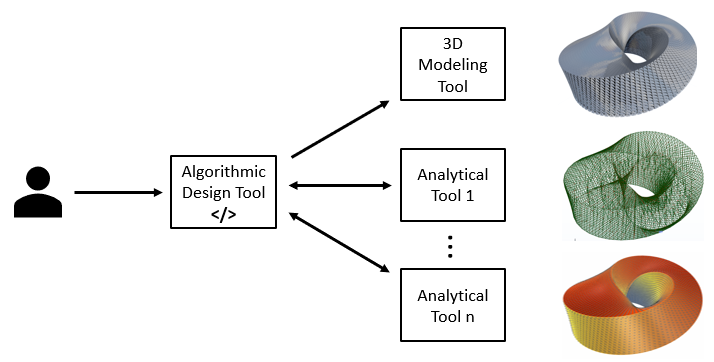
\includegraphics[width=0.90\textwidth]{./Images/Introduction/AlgorithmicDesignAndAnalysis_w_models.png}
\caption[General view of the Algorithmic Design and Analysis design approach]{Algorithmic Design and Analysis design workflow with examples of the Astana's National Library design and analytical models: (top) 3D model; (center) Robot's structural analysis model; (bottom) Radiance's pos-radiation analysis model.}
\label{fig:algorithmicanalysis}
\end{figure}		
	
	The \ac{AA} approach is able to enhance performance-based design approaches, as it provides means to effortlessly perform analysis throughout the whole design process, instead of just at final stages. Depending on the performance requirements, architects might need to use different analysis tools: (1) for daylight analysis, DAYSIM and Radiance are very popular among the community, (2) for energy simulations, EnergyPlus, TRNSYS and DOE-2 are widely used~\cite{Nguyen2014}, (3) for structural analysis, Robot Structural analysis is a well-known reputed tool, and (4) Olive Tree Lab and Pachyderm Acoustical Simulation are examples of good acoustic analysis tools. 

	Together with \ac{AD}, \ac{AA} makes it possible to implement automated optimization processes, as it provides the mechanisms to quickly update a design, to generate the corresponding analytical model, and, finally, to automatically evaluate the design in an analytical tool. The optimization processes use the results produced by performance analysis tools for different variations of the design as the functions to optimize. 
	
% #############################################################################
\subsection{Architectural Optimization Workflow}

In this section, we discuss the different tasks involved in an \ac{AD}-based design workflow optimization process. We adopt the algorithmic-based workflow due to its growing popularity among the architectural community~\cite{Kestelier2013}, its parametrics models inherent flexibility, and its ability to automate the \textit{update-generate-evaluate} process. 

	When following an algorithmic-based design approach, the architect idealizes a design which he ought to produce in the corresponding \ac{AD} tool. For this purpose, he creates the computational program, defining the parameters that represent the degrees of freedom in his design, i.e., the parameters which he is willing to manipulate in order to achieve more efficient designs. After the conception of the design's algorithmic model and provided the values for the parameters, the \ac{AD} tool generates 3D or analytical models for visualization and performance analysis purposes, respectively. Optionally, the architect may decide to optimize his design according to some particular aspects, potentially leading to the exploration of design solutions that were not previously considered. In that case, the optimization algorithm explores different design candidates, using the results produced by simulation tools as the functions to optimize. The execution of the optimization algorithm then yields optimal (or near optimal) design solutions.
	
	Considering the previous view of an algorithmic-based design workflow, we identify four key dimensions in an optimization process:
	
% ------- BEGIN \ --------
\begin{enumerate}
% ANALYTICAL MODELS
\item \textbf{Analytical models}: when the optimization algorithm specifies a candidate design, i.e., a concrete configuration for the parameters of the model, analytical models are automatically generated by the \ac{AD} tool. These models are then used as input for the corresponding analytical tools. These models can be improved, either through simplification of the analytical models, or by enriching them with context information. The former enables the simplification of the analysis itself and potentially reduces the simulation time, by providing an equivalent but simpler model to the tool, whilst the latter enables the attainment of a more detailed and realistic simulation, which is not always possible due to limitations in the \ac{AD} tool. 

% OPTIMIZATION ALGORITHM
\item \textbf{Optimization algorithms}: the algorithms that explore the design space in the quest for optimal (or near optimal) solutions. These algorithms use the results obtained from performance analysis of different design variations as the functions to optimize, i.e., as objective functions. Generally, the algorithm uses these inferred functions to guide the search for optimal solutions. The time complexity of the algorithm is typically dependent on the number of function evaluations. In architectural design, these functions entail time-intensive simulations, thus instilling optimization processes that may take minutes, hours, days, or even weeks to complete.

% EXPLAINABILITY / INTELLIGIBILITY OF RESULTS
\item \textbf{Intelligibility of Results}: Cichocka et al. identify the need for intelligibility of the optimization processes within the architectural community \cite{Cichocka2017SURVEY}. Having access to an explanation regardig the quality of a design solution allows architects to make more informed decisions. With these explanations, the archtiect can not only provide valuable arguments for its implementation, but also, depending on the quality of the explanations, learn with the process, thus fostering more efficient and faster future designs. 

% INTERACTIVITY AND VISUALIZATION
\item \textbf{Interactivity and Visualization}: interactive and visual aspects are highly important features in the context of an optimization process~\cite{Ashour2015CreativelyMOO}. On the one hand, an interactive optimization process enables its user to transfer knowledge about the problem at hand, for instance, by adding or removing constraints or by exploring different, yet unexplored regions of the design space, hence potentially increasing this process' performance. On the other hand, optimization processes providing better visualizations and representations of their own evolution can present their users with better feedback about the course of the search. This feedback is important, as it also allows the comparison of variable-objective correlations and the making of more informed decisions about the optimization process itself, e.g., whether the evaluations made so far suffice or if the algorithm is converging to non-conventional designs that he refuses to accept.
\end{enumerate}


% #############################################################################
\section{Goals}
The interest in design optimization is evident within the architectural community, however the currently existing tools are often fragile or limited, frequently compromising the application of optimization in architecture. This thesis focus on optimization processes within the architectural domain, providing a framework for optimizing both single and multi-objective problems. The implementation of such framework requires the definition of: (1) a modeling language to support the specification of optimization problems, (2) a wide variety of optimization algorithms to solve optimization problems, and (3) a visual presentation of the obtained results to provide a more comprehensible feedback over the optimization results.

To achieve the goals that we proposed to, we reviewed different mathematical optimization modeling languages and optimization frameworks, pondering the benefits and obstacles of each one. Based on these languages and frameworks, we established the basis requirements for the framework that enable its seamless application within the architectural practice. 

% #############################################################################
\section{Organization of the Document}
This thesis is is organized as follows: \Cref{chap:intro} discusses optimization concepts and evidences its importance for different problems, ranging from simpler day-to-day decisions to more complex engineering problems, such as components, circuits, and building designs. Particularly, this chapter stresses the relevance of optimization in the architectural context, providing a comprehensive overview of the existing practices and the difficulties underlying the adoption of optimization processes in architecture.
In \cref{chap:back}, we provide an overview over the currently existing optimization practices in architecture and we make a balance of the benefits and drawbacks associated to each one. 
In \cref{chap:architecture}, we describe the architecture of the implemented frameworks and we enumerate important design decisions that were made during this work.
\Cref{chap:evaluation} comprises both the quantitative and qualitative evaluations of the proposed solution, evaluating its performance in the context of three real-world case studies. 
\Cref{chap:conclusion} emphasizes the importance of optimization in architecture and draws some conclusions about the final work and how it effectively can influence the optimization practice. Finally, we reflect over future improvements for the proposed frameworks.
